\documentclass[a4paper, oneside]{book}
\usepackage[utf8]{inputenc}
\usepackage{csquotes}
\usepackage{graphicx} % allows inserting graphics
\graphicspath{ {./screenshot/} }
\usepackage{algpseudocode} % allows code snippets
\usepackage{algorithm} 
\usepackage{hyperref} % aggiunge collegamenti ipertestuali
\usepackage{zref-xr} % permette riferimenti incrociati: definire prima l'hyperref e poi il label a cui si riferisce.
\usepackage{subcaption} 
\usepackage[export]{adjustbox} 
\usepackage{wrapfig} % allows warped figures
\usepackage[acronym]{glossaries} % add glossary
\usepackage{acronym} % add acronyms
\usepackage{subfiles} % support multiple files
\usepackage{fancyhdr} % more control on headers and footers
\usepackage[italian]{babel} % mette la lingua italiana
\usepackage{underscore} % Permette di usare gli underscore senza che vengano riconosciuti come caratteri speciali
\setcounter{tocdepth}{4} % Permette di visualizzare le subsubsection nell'indice
\usepackage{listings} 
\lstset{
    showspaces=false, % non mostrare gli spazi come simboli
    showstringspaces=false, % non mostrare gli spazi all'interno di stringhe
    showtabs=false % non mostrare le tabulazioni come simboli
}

% Definisce i colori che si possono utilizzare
\usepackage{xcolor} 
\usepackage[table]{xcolor}
\colorlet{punct}{red!60!black}
\definecolor{background}{HTML}{EEEEEE}
\definecolor{delim}{RGB}{20,105,176}
\colorlet{numb}{magenta!60!black}

\usepackage{color}

\definecolor{dkgreen}{rgb}{0,0.6,0}
\definecolor{gray}{rgb}{0.5,0.5,0.5}
\definecolor{mauve}{rgb}{0.58,0,0.82}
\definecolor{lightgray}{rgb}{.9,.9,.9}
\definecolor{darkgray}{rgb}{.4,.4,.4}
\definecolor{purple}{rgb}{0.65, 0.12, 0.82}

% Definisce i colori per i json
\lstdefinelanguage{json}{
    basicstyle=\ttfamily\scriptsize,
    %numbers=left,
    %numberstyle=\scriptsize,
    %stepnumber=1,
    %numbersep=8pt,
    showstringspaces=false,
    breaklines=true,
    frame=lines,
    %backgroundcolor=\color{background},
    literate=
      {:}{{{\color{punct}{:}}}}{1}
      {,}{{{\color{punct}{,}}}}{1}
      {\{}{{{\color{delim}{\{}}}}{1}
      {\}}{{{\color{delim}{\}}}}}{1}
      {[}{{{\color{delim}{[}}}}{1}
      {]}{{{\color{delim}{]}}}}{1},
}

\lstdefinelanguage{typescript}{
  keywords={typeof, new, true, false, catch, function, return, null, catch, switch, var, if, in, while, do, else, case, break},
  keywordstyle=\color{blue}\bfseries,
  ndkeywords={class, export, boolean, throw, implements, import, this},
  ndkeywordstyle=\color{darkgray}\bfseries,
  identifierstyle=\color{black},
  sensitive=false,
  comment=[l]{//},
  morecomment=[s]{/*}{*/},
  commentstyle=\color{purple}\ttfamily,
  stringstyle=\color{red}\ttfamily,
  morestring=[b]',
  morestring=[b]"
}

\lstset{frame=tb,
  language=Java,
  aboveskip=3mm,
  belowskip=3mm,
  showstringspaces=false,
  columns=flexible,
  basicstyle={\small\ttfamily},
  numbers=none,
  numberstyle=\tiny\color{gray},
  keywordstyle=\color{blue},
  commentstyle=\color{dkgreen},
  stringstyle=\color{mauve},
  breaklines=true,
  breakatwhitespace=true,
  tabsize=3
}

\pagestyle{plain} %oppure none
% Altrimenti usare fancy header per più controllo: 
%https://www.overleaf.com/learn/latex/Headers_and_footers#Using_the_fancyhdr_package

% Per generare la bibliografia
\usepackage[
backend=biber,
style=ieee,
sorting=none 
%sorting=ynt
]{biblatex}
\addbibresource{files/bibliografia.bib}

%\makeglossaries 

 % Numerazione delle prima pagina con i numeri romani
\pagenumbering{roman}

\newglossaryentry{latex}{name=latex,
    description={Is a markup language specially suited for 
scientific documents}}
 
% Inizio del documento
\begin{document}

% Prima pagina di template
\subfile{files/frontespizio.tex}

\tableofcontents
\listoffigures
%\listoftables
%\printglossary
\clearpage
% \chapter*{Acronyms}
% \begin{acronym}
% \acro{gcd}{GCD}{Greatest Common Divisor}  
% \end{acronym}

% Numera le pagine con i numeri arabi e resetta il counter da questa pagina in poi
\pagenumbering{arabic} 
\setcounter{page}{1}
 
% File di introduzione
\subfile{files/introduzione.tex} 

% Capitolo 1 - Tecnlogie Utilizzate
\subfile{files/corpo/capitolo1.tex}
 
% Capitolo 2 - Approccio proposto
\subfile{files/corpo/capitolo2.tex}

% Capitolo 3 - Sviluppo
\subfile{files/corpo/capitolo3.tex}

% Capitolo 4 - Idee future
\subfile{files/corpo/capitolo4.tex}

% Capitolo 5 - Ulteriori cose sviluppate non riguardanti i meeting
\subfile{files/corpo/capitolo5.tex}

% \chapter{Step2: Text style}
% \section{Bold}
% Example of bold \textbf{text}.
% \section{Italic}
% Example of italic \textit{text}.
% \section{Underline}
% Example of underlined \underline{text}.
% \section{mixed}
% Example of mixed \textbf{\textit{word}}
% \section{emph}
% \textbf{Example of emph \emph{word}}\\
% \textit{Example of emph \emph{word}}

% \chapter{Elements of the document}
% \section{Images}


% \begin{figure}[H]
% \centering
% 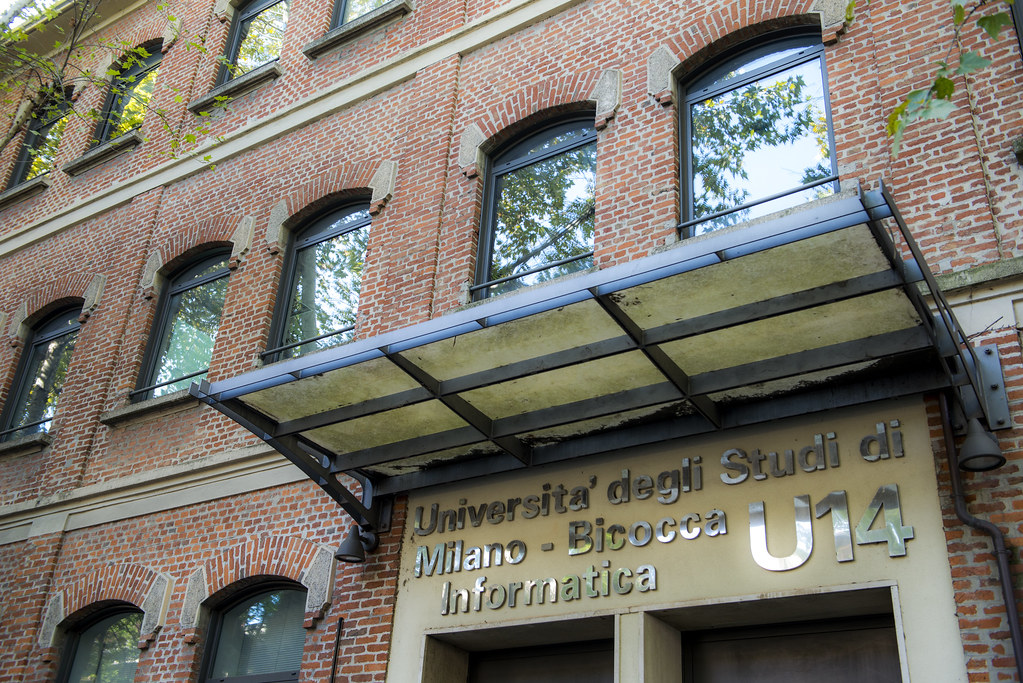
\includegraphics[width=0.5\textwidth]{images/u14.jpg}
% \caption{Example image}
% \label{img:ref_image}
% \end{figure}

% Reference to the image \ref{img:ref_image}.

% \section{Tables}
% \begin{table}
% \centering
% \begin{tabular}{|c|c|c|} 
%  \hline
%  cell1 & cell2 & cell3 \\ \hline
%  cell4 & cell5 & cell6 \\ \hline
%  cell7 & cell8 & cell9 \\ \hline
% \end{tabular}
% \caption{Example table}
% \label{tab:ref_table}
% \end{table}

% Reference to the table \ref{tab:ref_table}.

% \section{List}
% Example of an unordered list:
% \begin{itemize}
%   \item List entries start with the \verb|\item| command.
%   \item Individual entries are indicated with a black dot, a so-called bullet.
%   \item The text in the entries may be of any length.
% \end{itemize}

% Example of an ordered list:
% \begin{enumerate}
%   \item This is the first entry in our list.
%   \item The list numbers increase with each entry we add.
% \end{enumerate}

% Example of nested list:
% \begin{enumerate}
%    \item First level item
%    \item First level item
%    \begin{enumerate}
%      \item Second level item
%      \item Second level item
%      \begin{enumerate}
%        \item Third level item
%        \item Third level item
%        \begin{enumerate}
%          \item Fourth level item
%          \item Fourth level item
%        \end{enumerate}
%      \end{enumerate}
%    \end{enumerate}
%  \end{enumerate}


% \section{Equations}

% This is an example of an in-line equation: $E = MC^2$\\
% This is an example of an display mode equation:
% \begin{equation}
%     E = MC^2
% \label{eq}
% \end{equation}

% This is a reference to the Equation \ref{eq}.

% \section{Code Snippet}

% \subsection{verbatim}
% \begin{verbatim}
% Text enclosed inside \texttt{verbatim} environment 
% is printed directly 
% and all \LaTeX{} commands are ignored.
% \end{verbatim}

% \subsection{listings}
% \begin{lstlisting}
% import numpy as np
    
% def incmatrix(genl1,genl2):
%     m = len(genl1)
%     n = len(genl2)
%     M = None #to become the incidence matrix
%     VT = np.zeros((n*m,1), int)  #dummy variable
    
%     #compute the bitwise xor matrix
%     M1 = bitxormatrix(genl1)
%     M2 = np.triu(bitxormatrix(genl2),1) 

%     for i in range(m-1):
%         for j in range(i+1, m):
%             [r,c] = np.where(M2 == M1[i,j])
%             for k in range(len(r)):
%                 VT[(i)*n + r[k]] = 1;
%                 VT[(i)*n + c[k]] = 1;
%                 VT[(j)*n + r[k]] = 1;
%                 VT[(j)*n + c[k]] = 1;
                
%                 if M is None:
%                     M = np.copy(VT)
%                 else:
%                     M = np.concatenate((M, VT), 1)
                
%                 VT = np.zeros((n*m,1), int)
    
%     return M
% \end{lstlisting}

% \subsection{algpseudocode}
% \begin{algorithmic}
% \State $i \gets 10$
% \If{$i\geq 5$} 
%     \State $i \gets i-1$
% \Else
%     \If{$i\leq 3$}
%         \State $i \gets i+2$
%     \EndIf
% \EndIf 
% \end{algorithmic}

% \subsection{algorithm}

% reference to algorithm \ref{alg:cap}
% \begin{algorithm}[!h]
% \caption{An algorithm with caption}\label{alg:cap}
% \begin{algorithmic}
% \Require $n \geq 0$
% \Ensure $y = x^n$
% \State $y \gets 1$
% \State $X \gets x$
% \State $N \gets n$
% \While{$N \neq 0$}
% \If{$N$ is even}
%     \State $X \gets X \times X$
%     \State $N \gets \frac{N}{2}$  \Comment{This is a comment}
% \ElsIf{$N$ is odd}
%     \State $y \gets y \times X$
%     \State $N \gets N - 1$
% \EndIf
% \EndWhile
% \end{algorithmic}
% \end{algorithm}

% \section{href}
% For further references see \href{http://www.overleaf.com}{Something Linky} 
% or go to the next url: \url{http://www.overleaf.com}

% \chapter{Positioning and Size}

% \section{package adjustbox}
% 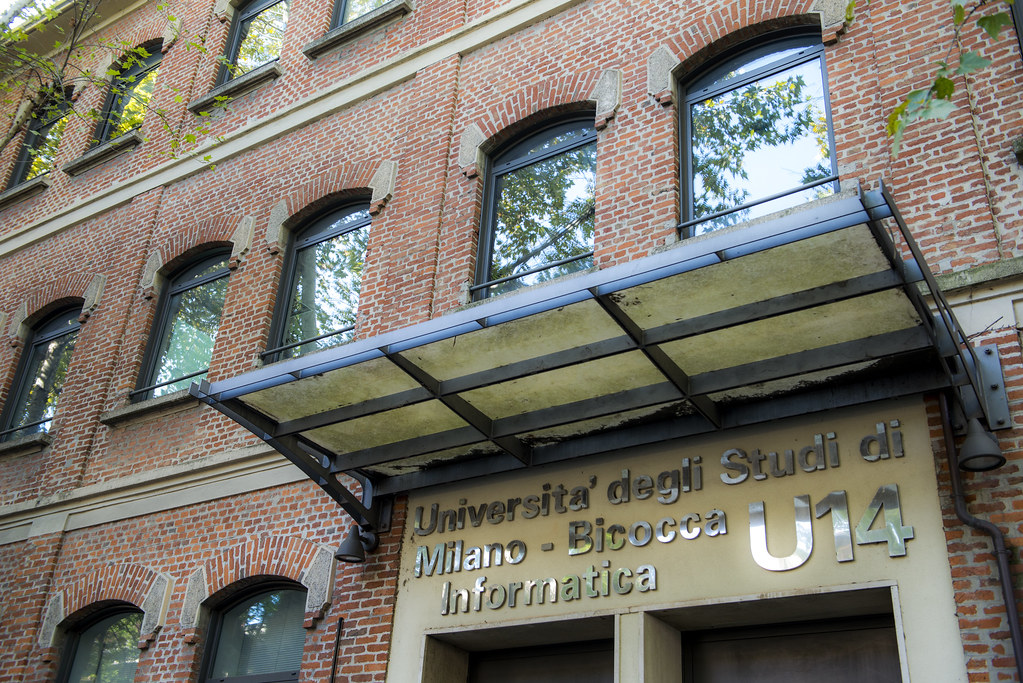
\includegraphics[width=0.5\textwidth, right]{images/u14.jpg}

% \section{Figure environment}

% \begin{figure}[h]
% 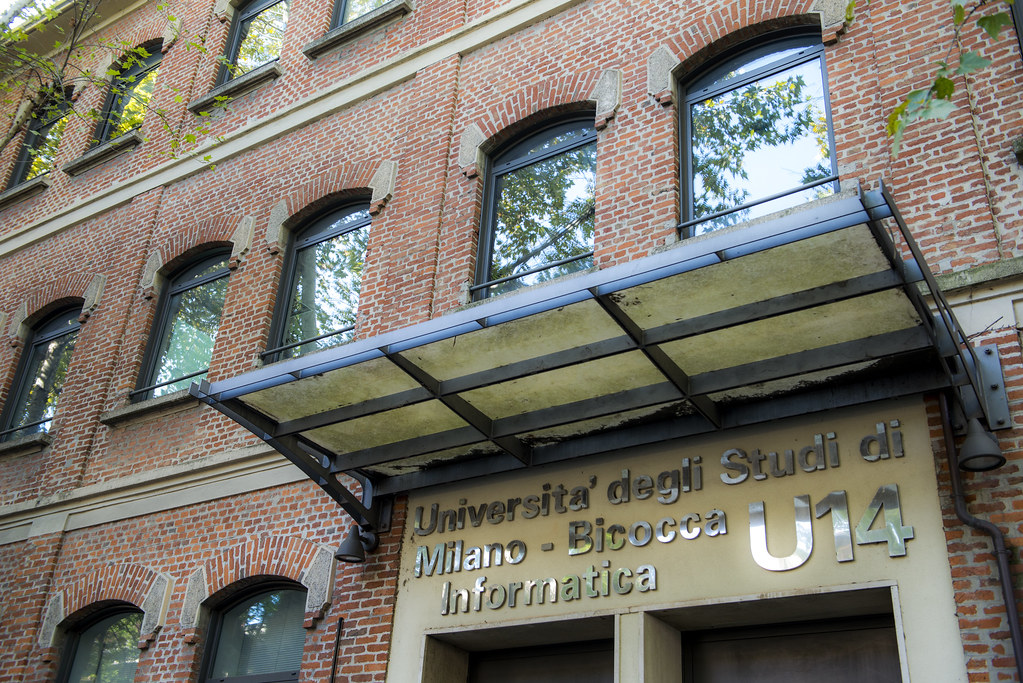
\includegraphics[width=0.5\textwidth, inner]{images/u14.jpg}
% \caption{h image}
% \label{fig:figure4}
% \end{figure}

% \begin{figure}[t]
% 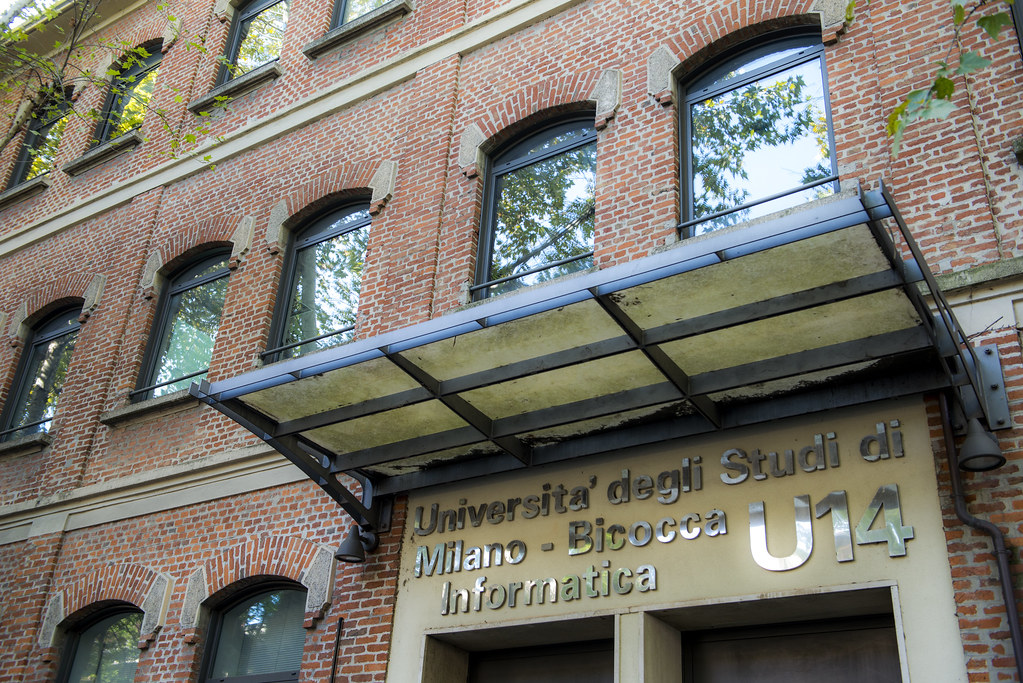
\includegraphics[width=0.5\textwidth, inner]{images/u14.jpg}
% \caption{Top image}
% \label{fig:figure2}
% \end{figure}

% \begin{figure}[!]
% 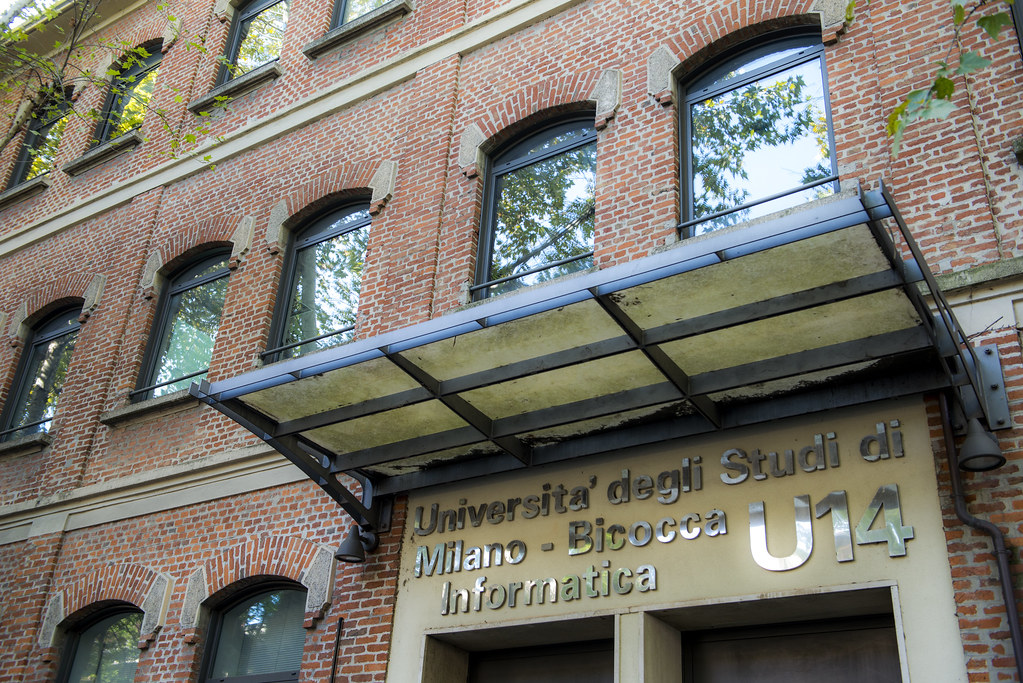
\includegraphics[width=0.5\textwidth, inner]{images/u14.jpg}
% \caption{! image}
% \label{fig:figure3}
% \end{figure}

% \chapter{Advanced images and table}

% \section{Double figures}
% Praesent in sapien. Lorem ipsum dolor sit amet, consectetuer adipiscing elit. Duis fringilla tristique neque...

% \begin{figure}[h]
% \begin{subfigure}{0.5\textwidth}
% 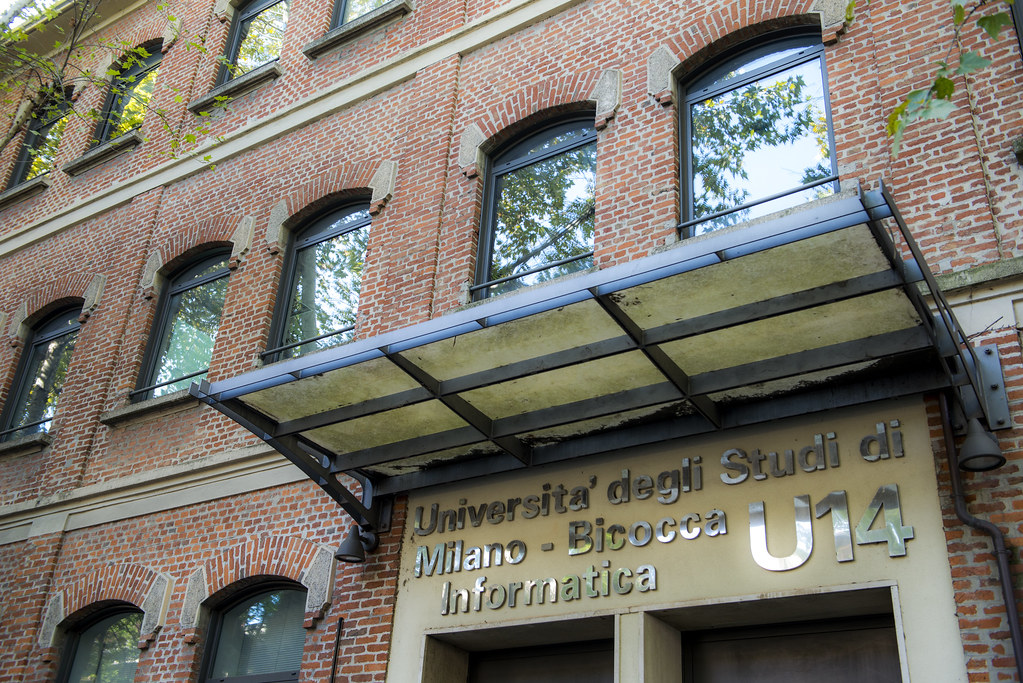
\includegraphics[width=0.9\linewidth, height=6cm]{images/u14.jpg} 
% \caption{Caption1}
% \label{fig:subim1}
% \end{subfigure}
% \begin{subfigure}{0.5\textwidth}
% 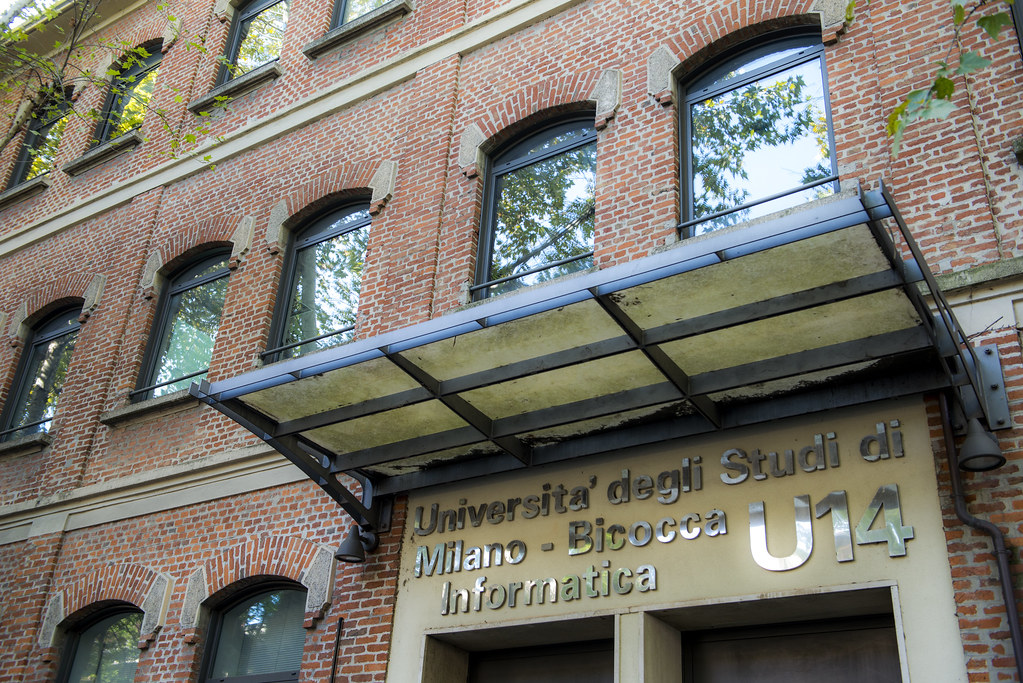
\includegraphics[width=0.9\linewidth, height=6cm]{images/u14.jpg}
% \caption{Caption 2}
% \label{fig:subim2}
% \end{subfigure}

% \caption{Caption for this figure with two images}
% \label{fig:image2}
% \end{figure}

% Praesent blandit blandit mauris. Praesent lectus tellus, aliquet aliquam, luctus a, egestas a, turpis. Mauris lacinia lorem sit amet ipsum. Nunc quis urna dictum turpis accumsan semper.

% \section{Wrapped images}

% Praesent in sapien. Lorem ipsum dolor sit amet, consectetuer 
% adipiscing elit. Duis fringilla tristique neque. Sed interdum 
% libero ut metus. Pellentesque placerat.

% \begin{wrapfigure}{l}{0.25\textwidth}
% 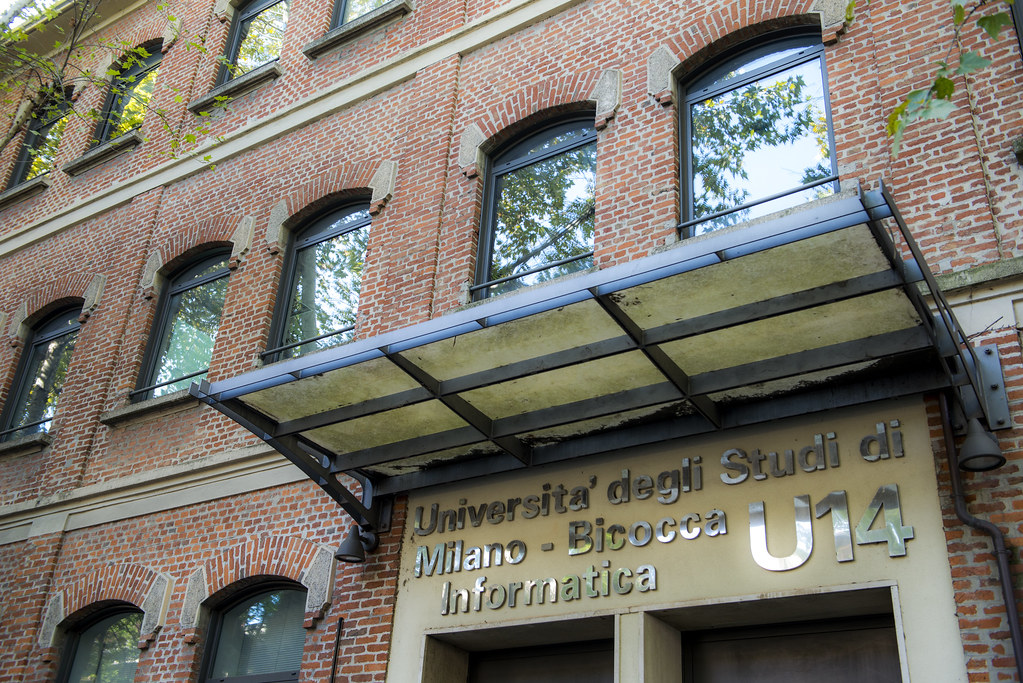
\includegraphics[width=0.9\linewidth]{images/u14.jpg} 
% \caption{Caption1}
% \label{fig:wrapfig}
% \end{wrapfigure}

% Praesent in sapien. Lorem ipsum dolor sit amet, consectetuer 
% adipiscing elit. Duis fringilla tristique neque. Sed interdum
% Lorem ipsum dolor sit amet, consectetur adipisici elit, sed eiusmod tempor incidunt ut labore et dolore magna aliqua. Ut enim ad minim veniam, quis nostrud exercitation ullamco laboris nisi ut aliquid ex ea commodi consequat. Quis aute iure reprehenderit in voluptate velit esse cillum dolore eu fugiat nulla pariatur. Excepteur sint obcaecat cupiditat non proident, sunt in culpa qui officia deserunt mollit anim id est laborum.
 
% \subsection{Wrapped Tables}
 
% Lorem ipsum dolor sit amet, consectetur adipisici elit, sed eiusmod tempor incidunt ut labore et dolore magna aliqua. Ut enim ad minim veniam, quis nostrud exercitation ullamco laboris nisi ut aliquid ex ea commodi consequat. Quis aute iure reprehenderit in voluptate velit esse cillum dolore eu fugiat nulla pariatur. Excepteur sint obcaecat cupiditat non proident, sunt in culpa qui officia deserunt mollit anim id est laborum.
% %------------------------------------------
% \begin{wraptable}{r}{5.5cm}
% \caption{A wrapped table going nicely inside the text.}\label{wrap-tab:1}
% \begin{tabular}{ccc}\  
% Header-1 & Header-1 & Header-1 \\
% 2 &3 & 5\\  
% 2 &3 & 5\\  
% 2 &3 & 5\\  
% \end{tabular}
% \end{wraptable}
% Lorem ipsum dolor sit amet, consectetur adipisici elit, sed eiusmod tempor incidunt ut labore et dolore magna aliqua. Ut enim ad minim veniam, quis nostrud exercitation ullamco laboris nisi ut aliquid ex ea commodi consequat. Quis aute iure reprehenderit in voluptate velit esse cillum dolore eu fugiat nulla pariatur. Excepteur sint obcaecat cupiditat non proident, sunt in culpa qui officia deserunt mollit anim id est laborum.

% \chapter{Additional concepts}

% \section{Terms} 

% The \Gls{latex} typesetting markup language is specially suitable 
% for documents that include maths. Formula are rendered 
% properly an easily once one gets used to the commands.

% \section{Acronym}

% Given a set of numbers, there are elementary methods to compute 
% its \ac{gcd}, which is abbreviated gcd. This 
% process is similar to that used for the lcm.

% \chapter{Multiple files management}
% \section{Multiple file 1}
% \subfile{multiple-files/file-one}

% \section{Multiple file 1}

% Aggiunge la bibliografia
\printbibliography
\addcontentsline{toc}{chapter}{\bibname}

% Aggiunge l'appendice
\appendix
\subfile{files/appendice.tex}

% Fine del documento
\end{document}